\documentclass[conference]{IEEEtran}
\IEEEoverridecommandlockouts
% The preceding line is only needed to identify funding in the first footnote. If that is unneeded, please comment it out.
\usepackage{cite}
\usepackage{amsmath,amssymb,amsfonts}
\usepackage{algorithmic}
\usepackage{graphicx}
\usepackage{textcomp}
\usepackage{xcolor}
\usepackage{hhline}
\def\BibTeX{{\rm B\kern-.05em{\sc i\kern-.025em b}\kern-.08em
    T\kern-.1667em\lower.7ex\hbox{E}\kern-.125emX}}
\begin{document}

\title{Peak Shaving with Bifacial Solar PV: Simulated Storage Battery Dispatch for Electric Vehicle Charging}

\author{\IEEEauthorblockN{1\textsuperscript{st} Given Name Surname}
\IEEEauthorblockA{\textit{dept. name of organization (of Aff.)} \\
\textit{name of organization (of Aff.)}\\
City, Country \\
email address or ORCID}
\and
\IEEEauthorblockN{2\textsuperscript{nd} Given Name Surname}
\IEEEauthorblockA{\textit{dept. name of organization (of Aff.)} \\
\textit{name of organization (of Aff.)}\\
City, Country \\
email address or ORCID}
\and
\IEEEauthorblockN{3\textsuperscript{rd} Given Name Surname}
\IEEEauthorblockA{\textit{dept. name of organization (of Aff.)} \\
\textit{name of organization (of Aff.)}\\
City, Country \\
email address or ORCID}
}

\maketitle

\begin{abstract}
Electric load peak shaving is a challenging and important problem considering the rapid growth of high-power electric vehicle charging sites. This novel study models vertically-oriented and West-facing bifacial solar photovoltaic modules to increase late afternoon production, and simulates peak shaving using a storage battery system. With occasional evening load peaks and a retail electric tariff with a 16:00-21:00 peak time of use period, this late afternoon production aligns both with load and with higher electric prices. Exploiting this, an electric load peak shaving simulator dispatches a stationary battery using a threshold-based approach, where the thresholds are optimized by a Newton-Raphson-based gradient descent method. The optimizer is verified to be within 0.1 $kW$. Five case studies and a sensitivity analysis on battery energy capacity and solar array configuration are considered. Relative to the base case, a total retail electric cost reduction of \$1422 (6.7\%) is achieved with a modest battery size of 25 $kWh$. Both data and code are shared with the public on GitHub.
\end{abstract}

\begin{IEEEkeywords}
Electric load, Peak shaving, Bifacial solar PV, EV charging.
\end{IEEEkeywords}

\section{Introduction}

% there will be peaks

\IEEEPARstart{T}{he} renewable energy transition will oversee a global shift toward electric energy consumption and renewable electric energy production in the coming decades. Since most electric transmission and distribution networks were built slowly over many decades, electric load growth will almost definitely outpace network upgrades. This is especially true for EV charging which coincides with existing peaks  \cite{Bobmann2015}, further decreasing the load factor ($P_{load,avg} P_{load,max}^{-1}$).

% load scheduling and solar peak-reduction

Consumers and fleets will be able to schedule charging for off-peak times and at lower power than the maximum and will do so if compensated or if charging is regulated. However public fast charging stations, among other cases, will often have a need to charge at high power and when the network is already near its peak. PV arrays, since they are not dispatchable, may stochastically reduce these peaks based on weather conditions, but also contribute to large transients in the net load, especially during peak load periods. This can be mitigated with nowcasting techniques that identify clouds with a 15-minute time horizon such as in \cite{Nespoli2022}. In many cases, dispatchable energy assets such as electric storage will still be required.

% battery peak shaving

Peak load management, referred to here as peak shaving, reduces load during periods of high load or high prices at a certain place in the network. Load curtailment, load re-scheduling, electric energy storage (battery or otherwise), or dispatchable DG are often employed \cite{Uddin2018}. Peaks may be defined statistically or maybe at a somewhat constant threshold. Grid operators may use peak shaving to increase power quality, defer future infrastructure upgrades, decrease losses, or reduce energy costs. Consumers may reduce their peaks for direct retail cost savings, but increasingly utilities and governments are compensating users to reduce peaks to defer infrastructure upgrades. Some carbon emission reduction is possible by reducing the on/off transitions of peaker plants due to load peaks \cite{Uddin2018}. A related problem is peak price management, which applies when market prices fluctuate naturally and is outside the scope of this study.

% cost function (move to method?)

% literature

In the literature, peak shaving papers often don't consider the retail cost of electricity and rarely utilize vertical bifacial solar PV or a threshold-based approach. In \cite{Reihani2016} authors forecast load and choose a State of Charge (SOC) trajectory to manage load peaks. Linear programming optimization in \cite{Lee2014} reduces the on-peak load of residential EV charging by dispatching a battery. In \cite{Gazafroudi2018} a multi-agent system buys and sells energy in a local energy market for a residence with solar PV and a dispatchable vehicle-to-home EV battery. In \cite{Zheng2015} authors optimized peak shaving based on a rate tariff and a technical power threshold. Vertical bifacial has been benchmarked in the literature and evaluated for new applications such as public highway solar installations \cite{Niccolai2022}. Vertical bifacial solar is coupled with a storage battery in \cite{Wallberg2022} and in \cite{Castellucci2022} with a rule-based peak shaving algorithm, reducing EV charging load peaks by 38.6\% and 79\%, respectively. However, the retail energy cost isn't estimated and a comparison is not made to understand the relative merit of vertical bifacial compared to south-facing modules. Bifacial PV has been studied extensively in the literature, performing around 11\% better than comparable monofacial PV \cite{Ogliari2023}.

% novelties

The main novelty of this study is analyzing the benefit of vertical bifacial solar in a peak shaving energy dispatch application, with a positive finding in certain cases. The cases consider different battery capacities, solar PV capacities, and solar PV arrays with different combinations of typical south-facing solar modules and vertical bifacial modules.  The product is a reproducible methodology implemented in Python, which is made available on GitHub along with time series and price data. 

\section{Methodology}

\begin{figure}
  \centering
  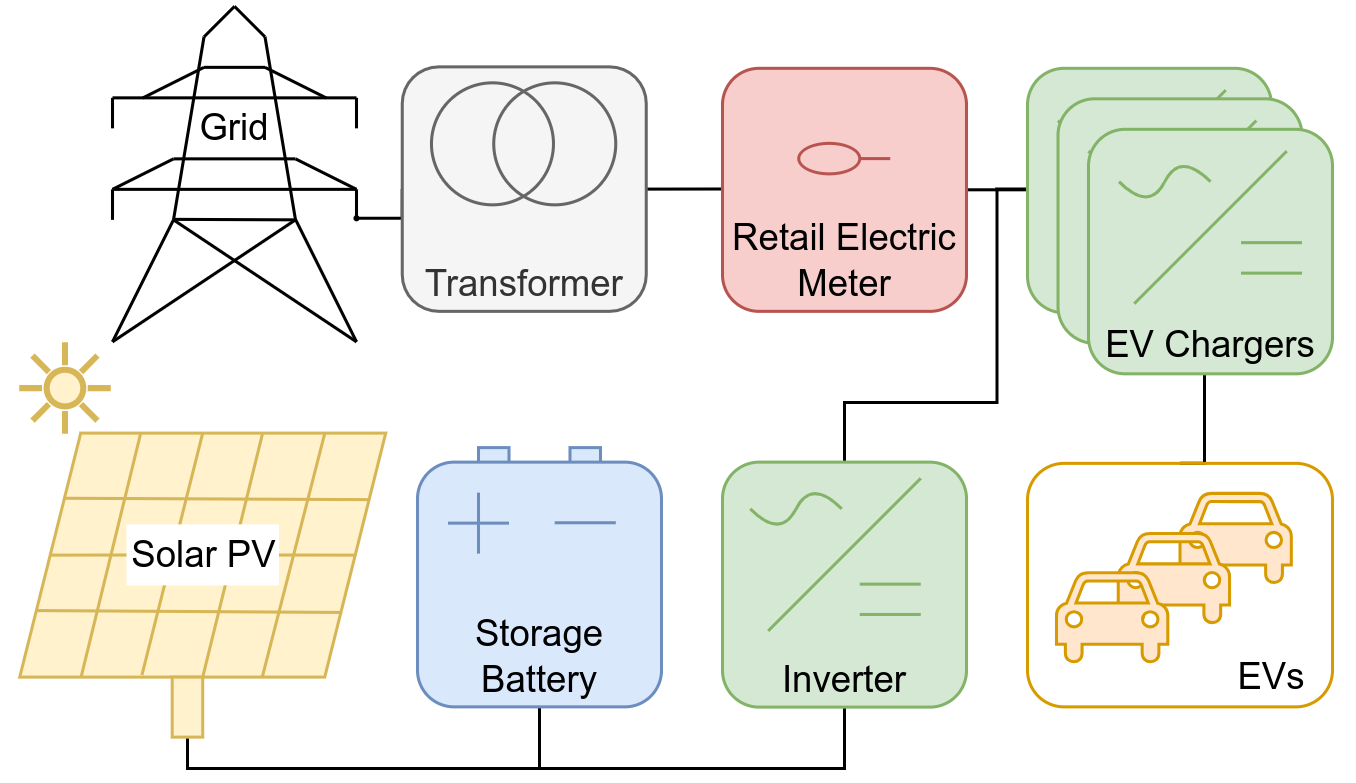
\includegraphics[width=1\linewidth]{images/oneline.png}
  \caption{Charging Site One Line Schematic. Simplified one-line schematic of the EV charging station with true measured EV charging power, modeled on-site solar generation, and a modeled stationary battery for economic peak shaving.}
  \label{fig:one-line}
\end{figure}

The methodology of this study is a set of energy dispatch computer simulations, mathematically formulated in Equation \ref{eq:peak-shaving}. We define the main power flow time series, all functions of discrete time, in units of $kW$, and $\in \mathbb{R}_0^+$:

\begin{itemize}
\item Load consumption: $ L(t) $%  \in \mathbb{R}_0^+ (kW)$
\item Solar production: $ S(t) $ %  \in \mathbb{R}_0^+ (kW)$
\item Battery discharge: $ B_d(t) $ % \in \mathbb{R}_0^+ (kW)  $
\item Battery charge: $ B_c(t) $ %\in \mathbb{R}_0^+ (kW) $
\item Net load: $ L_{net} = L - S$
\item Site load: $ L_{site} = L - S - B_d + B_c$
\item Peak shaving threshold: $ T(t) $ %   \in \mathbb{R}_0^+ (kW)  $ \\
\end{itemize}

A subscript $k$ for any variable denotes the TOU period to which it belongs, of $K$ total TOU periods. 

\subsection{Peak Shaving Algorithm}

Each simulation is performed on a month of time series data, stepping sequentially forward through the timesteps. If the net load is above the threshold $T$ the battery discharges at $L_{net}-T$. If the net load is below the threshold $T$ the battery charges at $T - L_{net}$. Essentially, the battery tries to maintain the site load as close as possible to the threshold, within its technical limits of power and energy capacity. 

At the beginning of a new month simulation, a gradient descent optimizer chooses the thresholds for each TOU period. The threshold is independent for each TOU period: if an electric tariff has three TOU periods (e.g. "peak", "mid-peak" and "off-peak") there will be different separate thresholds. 

\begin{align}
    \exists B_d, B_c\ & s.t.\ T\ = L-S-B_d+B_c, \forall\ t \label{eq:peak-shaving} \\
    & \text{subject to: } \notag \\
    B_d B_c  &= 0,\forall\ t  \\
    B_c, B_d  & \le B_{p,max},\forall\ t \\
    B_e(t)  & = B_{e,init} + \Delta t \Sigma_0^t{ [ B_c(t) \eta - B_d(t) \eta^{-1} ]} \label{eq:soc}
\end{align}
\begin{align*}
  %\begin{split}
    \notag
    & \text{where:} \\
    t & \in \{0, 0.25, 0.5, 0.75 ... t_{f}\} (h) \text{: time step}\\
    \Delta t & = 0.25 (h) \\
    B_{p,max} & \in \mathbb{R}_0^+ (kWh) \text{: battery maximum power } \\
    B_e(t) & \in \mathbb{R}_0^+ (kWh) \text{: state of charge } \\
    B_{e,init} & \in \mathbb{R}_0^+ (kWh) \text{: initial state of charge } \\
    B_{e,max} & \in \mathbb{R}_0^+ (kWh) \text{: battery energy capacity} \\
    \eta   & \in \mathbb{R}\ |\ 0<\eta<1 \text{: charge and discharge} \\
    & \text{ efficiency} \\    
  %\end{split}
\end{align*}

\subsection{Battery}

The battery is simulated with a minimum and maximum power and energy capacity, where the power capacity is 1C in all cases. State of charge $B_e$ is estimated by coulomb counting and a fixed half-cycle charging and discharging efficiency of 90\%, making the full-cycle efficiency 81\%. 

\subsection{Electric Tariff}

The electric tariff determines the total cost of electric service $C$, which is the sum of the monthly retail cost $C_m$. In this context, the main benefit of peak shaving is a reduction in the total cost to the consumer. See Equation \ref{eq:cost}. The energy cost is the energy delivered to the site multiplied by the energy price for that TOU period. The power cost is the monthly maximum of the 15-minute non-moving average site load for a certain TOU period, multiplied by the power price for that TOU period. Essentially, the energy cost is proportional to the area under the site load curve and the the power cost is proportional to the maximum monthly site load. 

\begin{align}
  %\begin{split}
    C_m           & = \sum_k^K [p_{p,k,m}  max(L^+_{site,k,m})] \label{eq:cost}\\
                  & + \sum_k^K [p_{e,k,m} \sum (L^+_{site,k,m}\Delta t) ] \notag \\
                  & \text{subject to:} \notag \\
                  L_{site,k,m}^+(t) & = L_{site}(t)\ \forall L_{site}(t)>0 
  \end{align}
\begin{align*}
                  & \text{where:} \\
                  k & \text{: TOU period} \\
                  K & \text{: total TOU periods} \\
                  m & \text{: month} \\
    C_m           & \in \mathbb{R}^+ (\$) \text{: monthly retail electric cost} \\
    p_{p,k,m}     & \in \mathbb{R}^+ (\$/kW) \text{: power price for TOU} \\
    p_{e,k,m}     & \in \mathbb{R}^+ (\$/kWh) \text{: energy price for TOU} \\
  %\end{split}
\end{align*}


\subsection{Threshold Optimizer}

The peak shaving thresholds (one per TOU period) are determined monthly by a custom gradient descent optimizer. The objective function \(C_m\) minimizes the retail energy cost of one month. See Equation \ref{eq:optimization}. Beginning from an initial guess the Newton-Raphson-based optimizer calculates the batch gradient and updates parameters based on a learning rate of 0.01 \cite{Truong2019}. This continues until the stopping condition is met, minimum cost for a patience of 50 iterations. This method is preferred over linear programming because it will minimize a variety of cost functions without needing to reformulate the linear program for each specific case study.

\begin{align}
    min[C_m(B_c,B_d)] & = min[C_m(T_1,T_2,..T_K)] \label{eq:optimization} \\
                      & \text{subject to: } \notag \\
    B_c(t)            & \le B_{p,max}  \\
    B_d(t)            & \le B_{p,max}  \\
    0         & \le B_{e}(t) \le B_{e,max} 
\end{align}

\subsection{Time Series Data}

All time series data is average real power over a 15-minute interval or is mean-downsampled to that interval. Timestamps are ISO-8601 format and beginning-of-period convention, so the 15-minute interval 1 January 2019 13:00:00 to 13:14:59 is labeled 2019-1-1T13:00 (the T can optionally be a space). All timestamps are in local time to avoid a +1-hour shift in the load profile during daylight savings time (summer). To avoid missing and repeated timestamps, the winter-spring missing hour is filled with 1-hour persistence, and the summer-fall extra hour is removed. The solar production data, which normally comes in standard time, is then shifted ahead 1 hour during daylight savings time, such that the timestamps match the load. This treatment is important since an unintentional 1-hour shift in the data can have large consequences on the temporal alignment of load and solar peaks. Also, electric tariff TOU periods are defined by local, not standard time. 


\subsection{Simulations}

One simulation solves the peak shaving problem for a month for a certain solar, battery, and load configuration. The result is a battery dispatch time series, one threshold value per TOU period, and a total cost for the month, $C_m$. The simulation process is explained in Figure \ref{fig:simulation-flowchart}. The simulation is repeated for every month of data and for various different solar and battery configurations. The implementation is Python 3.11 in Windows 10 64-bit, on an Intel i9 CPU with 64 GB of RAM.

\begin{figure}
    \centering
    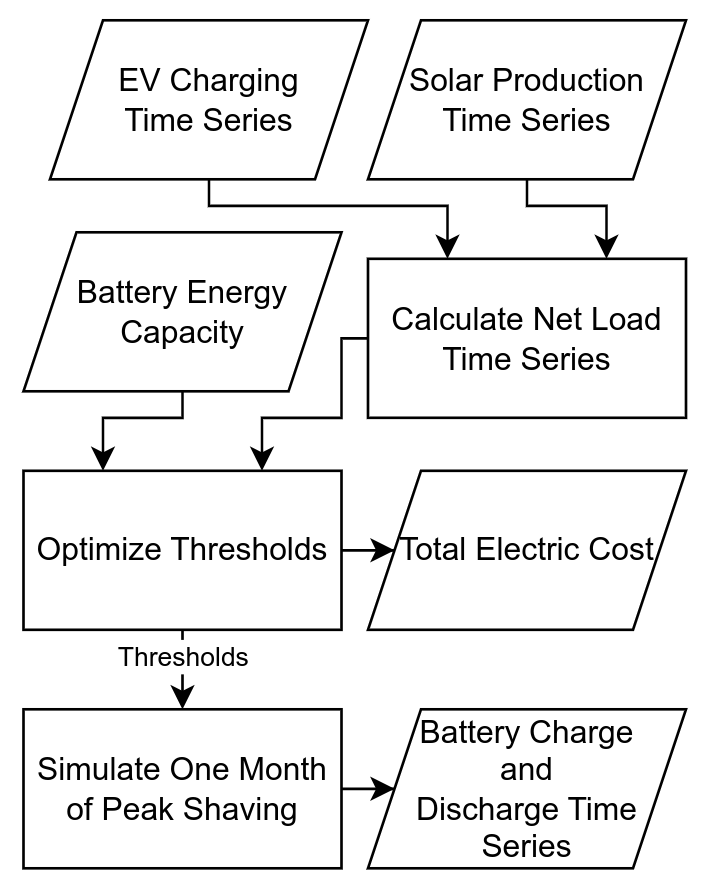
\includegraphics[width=0.6\linewidth]{images/simulation flowchart.png}
    \caption{Simulation Flowchart. For each solar array case, battery capacity, and set of power thresholds, a single simulation is performed on the data 1 month at a time.}
    \label{fig:simulation-flowchart}
\end{figure}

\section{Case Studies}

Five case studies are simulated and analyzed, where each case is a solar array with a different configuration of typical south-facing solar modules and west-facing vertical bifacial modules. The first case is a base case and the cost reductions of the other four cases are referred to this. See Table \ref{tab:casestudies}.

\begin{table}
  \centering
  \caption{Case Studies. All cases have the same total number of modules, but in cases 1-4 some percentage of modules are oriented west and tilted vertically. }
  \label{tab:casestudies}
  \setlength{\tabcolsep}{3pt}
  \begin{tabular}{@{}p{0.4cm} @{}p{2cm} l l l l l@{}}
    \hline
    N. & \textbf{Case Study}       & Capacity & Azimuth & Tilt & Solar Prod. \\
       &                           & $(kW_p)$ &         &      & ($MWh$)     \\
    \hhline {= = = = = =}
    1  & \textbf{South 20° (base)} & 129      & South   & 20°  & 151.7       \\
    \hline
    2  & \textbf{25\% West 90°}    & 97       & South   & 20°  & 146.5       \\
       &                           & 32       & West    & 90°  &             \\
    \hline
    3  & \textbf{50\% West 90°}    & 64       & South   & 20°  & 141.1       \\
       &                           & 64       & West    & 90°  &             \\
    \hline
    4  & \textbf{75\% West 90°}    & 32       & South   & 20°  & 136.1       \\
       &                           & 97       & West    & 90°  &             \\
    \hline
    5  & \textbf{100\% West 90°}   & 129      & West    & 90°  & 131.0       \\
    \hline
  \end{tabular}
\end{table}

The electric load time series is the same for each case and is measured EV charging power ("load") from the Caltech Adaptive Charging Network database at the Jet Propulsion Lab (JPL) in Pasadena, California \cite{Lee2021}. EV charging session data were usually available as a 10s-interval time series and was mean-downsampled to a 15-minute interval. For some sessions, the time series was not available and was instead estimated. The data range is from 2018-5-1 00:00 to 2019-2-28 23:45, so COVID-19 effects are not present. 

The solar production time series is different for each case, and all were modeled from GOES satellite irradiance data\cite{Sengupta2018}. The 5-minute interval multi-channel data are converted to irradiance by the FARMS \cite{Sengupta2018} radiation model and tilted to the plane of arrival by the REST2 \cite{gueymard2008rest2} model, producing irradiance components of DNI, DHI, and GHI. These functions are all implemented in the software System Advisor Model \cite{blair2018system}. 

The electric tariff is also the same for each case and is typical for California, consisting of several different TOU periods and both energy and power prices. In defining the tariff we use "h14-16" to mean 14:00-15:59" and 24h to mean 0:00-23:59. In parenthesis is the count of TOU periods for each season. Since the first "All seasons 24h" price of 26.07 $\$/kW$ applies to all hours of the day, any other TOU period's power price must be summed with that base price.

Electric tariff:
\begin{itemize}
\item \textbf{All seasons:} (1) 24h 26.07 \$/kW
    \item \textbf{Summer (Jun 1 - Sep 30):} (2) h0-14 \& h23-0  0.132 \$/kWh, (3) h14-16 \& h21-23 6.81 \$/kW \& 0.159 \$/kWh, (4) h16-h21 32.90 \$/kW \& 0.196 \$/kWh
    \item     \textbf{Winter (Oct 1 - Feb 28/29):} (2) h0-16 \& h21-0  0.132 \$/kWh, (3) h16-h21 2.22 \$/kW \& 0.172 \$/kWh
    \item \textbf{Spring (Mar 1 - May 31):} (2) h9-14 0.079 \$/kWh, (3) h0-h9 \& h14-16 \& h21-0 0.132 \$/kWh, (4) h16-h21 2.22 \$/kW \& 0.172 \$/kWh
\end{itemize}

Prices are highest in the summer and lowest in the spring, with the highest prices associated with the 16:00-21:00 period. This late afternoon and evening window is specifically when production from a typical South-facing 5 to 30° tilt is in a steep decline due to cosine losses. 


\section{Results}

The peak shaving methodology produces a retail electric cost for each of the 10 months of data. See Figure \ref{fig:total-cost} sums up the cost for each month and compares across case studies. The costs monotonically decrease with battery capacity as expected because every marginal unit of added battery energy capacity allows the algorithm to hold a power threshold for longer, and since each battery is rated for 1C at charging and discharging, the battery will also have more power capacity to achieve lower thresholds relative to the same size peak. Figure \ref{fig:total-cost-reduction} shows that the 100\% West 90° array achieves a lower total cost than the baseline South 20°. All three combination arrays achieve a lower cost for all battery capacities up to 200 $kWh$, with a maximum reduction of \$1422 (6.7\%) relative to the South 20° with a 100 $kWh$ battery. The largest percentage improvement of 7.10\% (\$1208) occurs for the same array and a 150 $kWh$ battery. The absolute cost reduction is likely more important than the relative reduction since it would be treated directly as revenue in a cash flow analysis to determine the economic performance of a given battery.

\begin{figure}
    \centering
    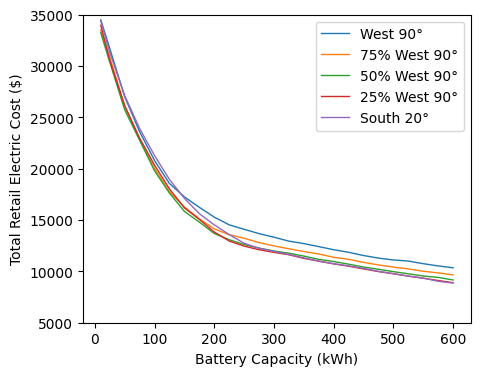
\includegraphics[width=0.75\linewidth]{images/total cost.png}
    \caption{Total Retail Electric Cost. Costs are calculated for each case study and a sensitivity analysis is performed on battery capacity ($kWh$). Below 150 kW the South 20° and 100\% West 90° arrays have similarly high total costs, whereas the three combination arrays are somewhat grouped a few percent below. Above 150 kW the total costs for each case diverge somewhat, with the South 20° base case attaining the lowest cost for the 400 $kWh$ battery and larger.}
    \label{fig:total-cost}
\end{figure}

\begin{figure}
    \centering
    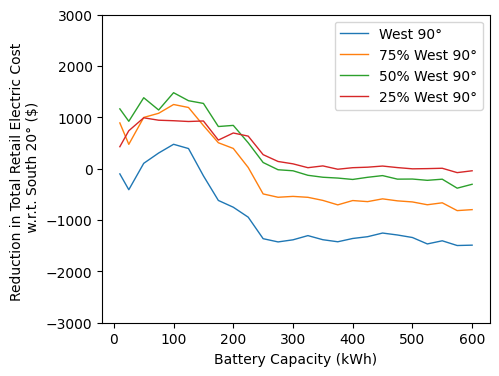
\includegraphics[width=0.75\linewidth]{images/total cost reduction.png}
    \caption{Reduction in Total Retail Cost is likely the most important metric for evaluating the peak shaving efficacy since it can be directly used as revenue in a cash flow analysis to calculate economic performance. The combination of the 50\% West 90° array and 100 $kWh$ battery achieved the largest cost reduction of \$1422 (6.7\%) over the 10-month data period.}
    \label{fig:total-cost-reduction}
\end{figure}
The benefit of vertical bifacial modules can be seen when comparing the simulated battery charge and discharge time series data. An example day (June 6) of peak shaving is chosen for the 100\% West 90° case in Figure \ref{fig:peak-shaving-west}, which is presented here as a clearer graphical example than the better-performing 50\% West 90° array. For both cases, June 6 is the limiting day for the month, when the battery reaches a technical limit, in these cases zero SOC. This is likely due to a particularly large evening peak load event from approximately 17:30 to 21:30, with a maximum power of 56 $kW$ and total energy of 201 $kWh$. For these simulations, the battery capacity is 125 $kWh$ nominal and 112.5 $kWh$ after losses, and as specified the battery will charge and discharge at a maximum of 1C or 125 $kW$. The base case of South 20° overproduces in the middle hours of the day and solar is exported to the network starting around 12:00. During the peak load event the South 20° only produces 18.8 $kWh$ whereas the 100\% West 90° array produces 104 $kWh$. In each case the battery charges to 100\% (125 $kWh$) before the evening peak load event. The result is that the evening net load peak in the 100\% West 90° case starts later and contains less energy, though it reaches the same maximum power. Due to this the battery in the 100\% West 90° case can hold the site load to a lower threshold in \(kW\), which is directly proportional to reducing the retail electric cost. During the expensive Peak TOU period of 14:00-21:00, the base South 20° case only achieves a low threshold of 13.0 $kW$, whereas the 100\% West 90° case holds a threshold of 3.1 $kW$ in the same period, a 76\% improvement. The retail electric cost isn't defined for only one day out of a typical month, since the power portion of the cost is calculated on the monthly peak. However if June 6 was the only day of the month with non-zero load the total cost would be \$983 for the South 20° case and \$560 for the 50\% West 90° case, which is a 43\% reduction.

\begin{figure}
    \centering
    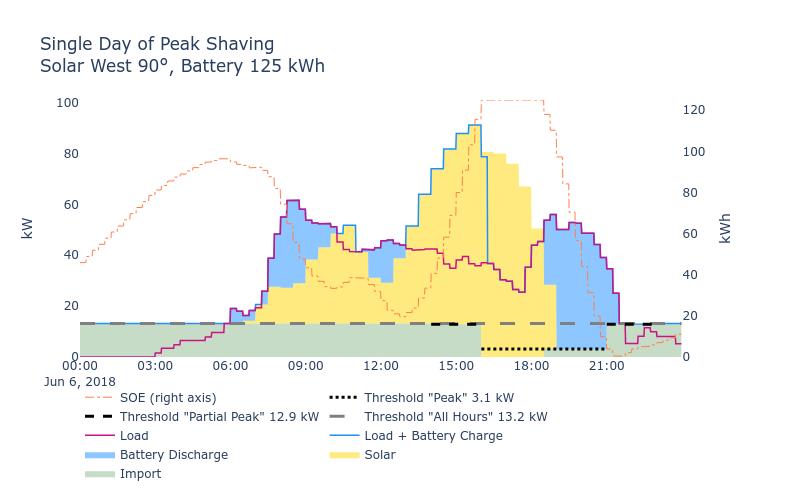
\includegraphics[width=1\linewidth]{images/single day of peak shaving west.png}
    \caption{Single Day of Peak Shaving (West 90° array). The 100\% West 90° case shifts production to the late afternoon, reducing the evening load energy and thereby the Peak period threshold to 7.7 $kW$, 42\% lower than the South 20° array.}
    \label{fig:peak-shaving-west}
\end{figure}
The largest cost reduction is \$1422 for the 50\% West 90° case and 100 $kWh$ battery. Note that the largest reduction in retail cost may not be the best solution economically, since the 25 $kWh$ battery achieves 65\% of the cost reduction at 20\% of the battery energy capacity, which is roughly proportional to capital cost.

A sensitivity analysis on the size of the solar array is performed with the results in Figure \ref{fig:solar-sensitivity} and Table \ref{tab:solar-sensitivity}. The total retail cost decreases monotonically with the larger solar capacities and the cost reduction increases by a factor of 10 from the smallest to largest solar capacity. This result is expected since the larger capacities create a more pronounced difference between the late afternoon production of the two arrays and the peak shaving strategy translates into lower power thresholds for the cases with some portion of the array in the 100\% West 90° orientation. The 50\% West 90° case performs best in the first four solar capacities at which point, for the first time, the best performing case is one where the majority of the modules are in the 100\% West 90° orientation (75\%). However, the difference of \$19 is not substantial. At larger solar capacities the cost reductions for each case study are both larger in magnitude and closer together, however, the increase in cost reduction is clearly less than linear with solar capacity. This suggests a diminishing returns problem where, after a certain capacity of 100\% West 90° modules is met, the additional South 20° and 100\% West 90° modules are providing energy when the battery is already at 100\% SOC.

\begin{table*}[h]
  \centering
  \caption{Solar Capacity Sensitivity Results. This analysis is based on a reduction in total retail cost relative to the base South 20° case. While the 50\% West 90° array continues to achieve the highest cost reduction, the battery capacity increases from 25 $kWh$ to 125 $kWh$.}
  \label{tab:solar-sensitivity}
  \begin{tabular}{ p{3cm} p{2cm} p{2cm} p{2.8cm} }
    \hline
    \textbf{Solar Capacity} $(kW_p)$ & \textbf{Best Case for Cost Reduction} & \textbf{Best Case Cost Reduction $(\$)$} & \textbf{Best Case Battery Capacity}
    $(\$)$                                                                                                                                                       \\
    \hline
    64.4 (0.5x)                         & 50\% West 90°                         & 260                                      & 25                                  \\
    128.8 (1.0x)                        & 50\% West 90°                         & 1422                                     & 100                                 \\
    193.2 (1.5x)                        & 50\% West 90°                         & 2211                                     & 125                                 \\
    257.6 (2.0x)                        & 75\% West 90°                         & 2579                                     & 125                                 \\
    \hline
  \end{tabular}
\end{table*}


\begin{figure}
    \centering
    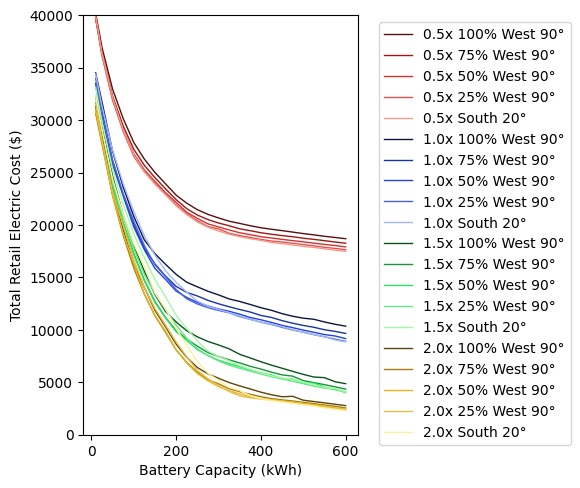
\includegraphics[width=1\linewidth]{images/total cost reduction solar sensitivity.png}
    \caption{Larger solar capacities monotonically reduce the cost for all cases, but the base case South 20° only marginally increases production during late afternoon peaks when the energy is needed.}
    \label{fig:solar-sensitivity}
\end{figure}

The battery capacities increase from 25 $kWh$ up to 125 $kWh$ across the solar sizes, which is an unexpected finding. Despite the extra capacity the 100\% West 90° case in Figure \ref{fig:weekly-load-solar} is still mostly unable to affect the peak power of the evening peaks, and thus both the base South 20° and combination array cases have a similar maximum power to shave. Indeed the average of the monthly peak net load values is 74.5 $kW$ for the South 20° 2.0x case and 74.7 $kW$ for the 100\% West 90° 2.0x case. However, when increasing the solar to 2.0x, the energy under the net load time series during the 17:00 to 22:00 period decreases by only 164 $kWh$ for the South 20° versus 886 $kWh$ for the 100\% West 90° case. With more solar production in the evening peak, the optimizer is able to pursue driving the "Peak" TOU period to zero, which has a large economic benefit. This is unachievable with the small battery capacities and is more difficult without the late afternoon solar production of the 100\% West 90° modules. Indeed a large 200 $kWh$ battery is required to achieve the first 0 $kW$ "Peak" period threshold in the South 20° case for all solar capacities. Rather, the 100\% West 90° case achieves a 0 $kW$ Peak period threshold with the 150 $kWh$ battery at 100\% solar capacity and with the 125 $kWh$ battery at 2.0x solar capacity.

\begin{figure}
    \centering
    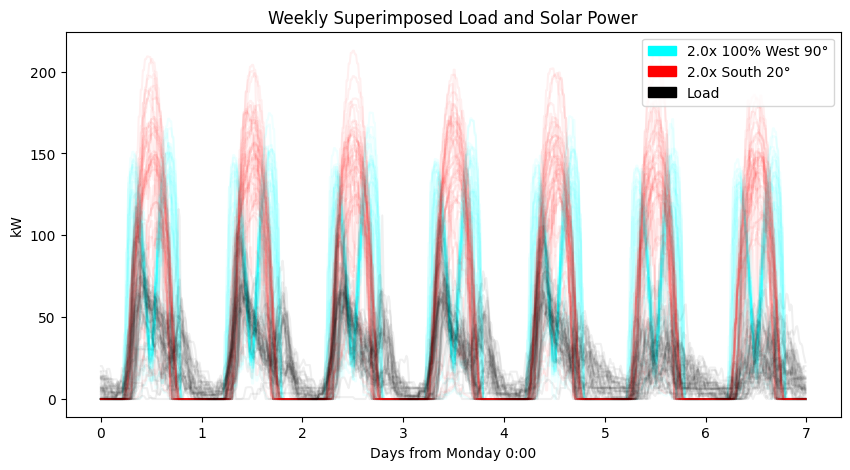
\includegraphics[width=1\linewidth]{images/weekly load solar.png}
    \caption{Weekly Overlaid Load and Solar Power. The entire 10-month time series of EV charging load, Solar 20°, and 100\% West 90° are superimposed on a weekly basis, beginning on Monday. The 100\% West 90° case provides a clearer graphical example than the better-performing cases.}
    \label{fig:weekly-load-solar}
\end{figure}

\section{Conclusions}

% This work simulates the benefit of vertically tilted West-facing bifacial solar modules in a peak shaving application. Peak shaving is achieved by an electric storage battery, a threshold-based algorithm, and a gradient descent optimizer. Five case studies are considered, all with the same real EV charging time series data. The variable in each case study is the percentage of bifacial solar modules that are West-facing and vertical, and which are South-facing and tilted at 20°.

The case studies are evaluated by the retail electric cost reduction relative to a base case of 100\% South 20° (0\% of modules are West 90°). The best-performing case is 50\% West 90°, achieving a reduction in the total retail cost of energy of \$1422 (6.7\%) with a 25 $kWh$ battery. While a vertical-bifacial array might have some benefit over the base case with no storage battery, solar power is inherently stochastic and therefore a single day of low solar can "set the peak of the month," which is multiplied in these case studies by a large power price during summer months especially. However, an interesting finding is that only a relatively small battery (25 $kWh$) relative to the load (maximum 117 $kW$) is required to fill the holes caused by the stochastic solar power profile. 

When solar is increased to twice the net-zero capacity the best-performing case is 75\% West 90° with a cost reduction of \$2579 (16.1\%) with a 125 $kWh$ battery. The best percentage cost reduction overall is 20.0\%. Generally, a larger solar capacity favors the vertical-bifacial arrays because the increase in the late afternoon is proportional to the solar capacity, but for the base case 0\% West 90° array the production is near zero at that time (so a proportional increase is still quite small). 

% Peak shaving a monthly peak power typically, depending on the load factor, results in dispatching the battery until its technical limits to achieve a minimum monthly peak power. Because the load, or net load after solar is dispatched, is often not very homogeneous there will be one limiting day where the battery is bound by its technical limits and the peak power of the month is set. The presence of this limiting day in the month simulation of Figure \ref{fig:peak-shaving} does not guarantee a global minimum cost, but the lack of a limiting day would suggest the global minimum was not found. Intuitively the limiting day can be thought of as the most difficult day for the battery to achieve the given thresholds, and if the day was somehow easier for the battery (less and more uniform net load) the power thresholds could be lowered and therefore a lower retail electric cost achieved. Because the results of each month typically depend strongly on one limiting day, small changes in the load or the solar power magnitude or temporal relationship can have a large impact on the overall results. For this reason, peak shaving simulations require particular care in data selection, cleaning, and acquiring an appropriately large amount of data such that the probability space of true possible limiting is well represented in the selected sample of limited days.

Confidence in the results presented is medium-high given the use of true EV charging measurements, a robust Newton-Raphson gradient descent optimizer, a true electric tariff appropriate for the load site and solar data location, and sensitivity analyses performed on two variables.

Future work should expand to other load data, include dynamic price for energy exported, utilize true solar production measurements, improve the battery state of charge estimation such as in \cite{Eleftheriadis2023}, perform simulations using forecasting load such as in \cite{Wood2023}, and test with hardware in the loop at the Politecnico di Milano MG2Lab microgrid.

\bibliographystyle{IEEEtran}
%\bibliographystyle{unsrt} %Bib in ordine di apparizione
\bibliography{mendeley}%} %nome Bib file in directory
\vspace{12pt}


\end{document}
